%%%%%%%%%%%%%%%%%%%%%%%%%%%%%%%%%%%%%%%%%
% Focus Beamer Presentation
% LaTeX Template
% Version 1.0 (8/8/18)
%
% This template has been downloaded from:
% http://www.LaTeXTemplates.com
%
% Original author:
% Pasquale Africa (https://github.com/elauksap/focus-beamertheme) with modifications by 
% Vel (vel@LaTeXTemplates.com)
%
% Template license:
% GNU GPL v3.0 License
%
% Important note:
% The bibliography/references need to be compiled with bibtex.
%
%%%%%%%%%%%%%%%%%%%%%%%%%%%%%%%%%%%%%%%%%

%----------------------------------------------------------------------------------------
%	PACKAGES AND OTHER DOCUMENT CONFIGURATIONS
%----------------------------------------------------------------------------------------

\documentclass[10pt]{beamer}
\usetheme{moloch}
%\setbeameroption{hide notes} % Only slides
%\setbeameroption{show only notes} % Only notes
\setbeameroption{show notes on second screen=right}

%\usetheme{focus} % Use the Focus theme supplied with the template
% Add option [numbering=none] to disable the footer progress bar
% Add option [numbering=fullbar] to show the footer progress bar as always full with a slide count

% Uncomment to enable the ice-blue theme
\definecolor{main}{RGB}{92, 138, 168}
\definecolor{background}{RGB}{240, 247, 255}

%------------------------------------------------
\usepackage[utf8]{inputenc}
\usepackage{booktabs} % Required for better table rules
\usepackage{tikz}
\usepackage{quiver}
\usepackage{url}
\usepackage{multicol}
\usepackage{esint}
\usepackage{amsfonts}
\usepackage{tikz}
\usetikzlibrary{decorations.pathmorphing}
\usepackage{amsmath,amssymb}
\usepackage{colortbl}
\usepackage{mathtools}
\usepackage{ mathrsfs }	
\usepackage{ dsfont }
\usepackage{ gensymb }
\usefonttheme{professionalfonts}
\setbeamerfont{bibliography item}{size=\footnotesize}
\setbeamerfont{bibliography entry author}{size=\footnotesize}
\setbeamerfont{bibliography entry title}{size=\footnotesize}
\setbeamerfont{bibliography entry location}{size=\footnotesize}
\setbeamerfont{bibliography entry note}{size=\footnotesize}

\newcommand{\R}{\mathbb{R}}
\newcommand{\Q}{\mathbb{Q}}
\newcommand{\C}{\mathbb{C}}
\newcommand{\Z}{\mathbb{Z}}
\newcommand{\N}{\mathbb{N}}
\newcommand{\F}{\mathbb{F}}
\newcommand{\Hom}{{\mathrm{Hom}}}
\newcommand{\image}{{\mathrm{Im}}}
\newcommand{\kernel}{{\mathrm{Ker}}}
\newcommand{\coker}{{\mathrm{coker}}}
\DeclareMathOperator*{\colim}{co{\lim}}
\DeclareMathOperator*{\hocolim}{hoco{\lim}}
\DeclareMathOperator*{\holim}{ho{\lim}}
\newcounter{dummy} \numberwithin{dummy}{section}

\newtheorem{proposition}[dummy]{Proposition}
\AtBeginSection[]{
	\begin{frame}
		\vfill
		\centering
		\begin{beamercolorbox}[sep=8pt,center,shadow=true,rounded=true]{title}
			\usebeamerfont{title}\insertsectionhead\par%
		\end{beamercolorbox}
		\vfill
	\end{frame}
}
%----------------------------------------------------------------------------------------
%	 TITLE SLIDE
%----------------------------------------------------------------------------------------

\title{Higher Algebraic K-Theory:\\ A simplicial approach}

\subtitle{}

\author{Bhoris Dhanjal}

%\titlegraphic{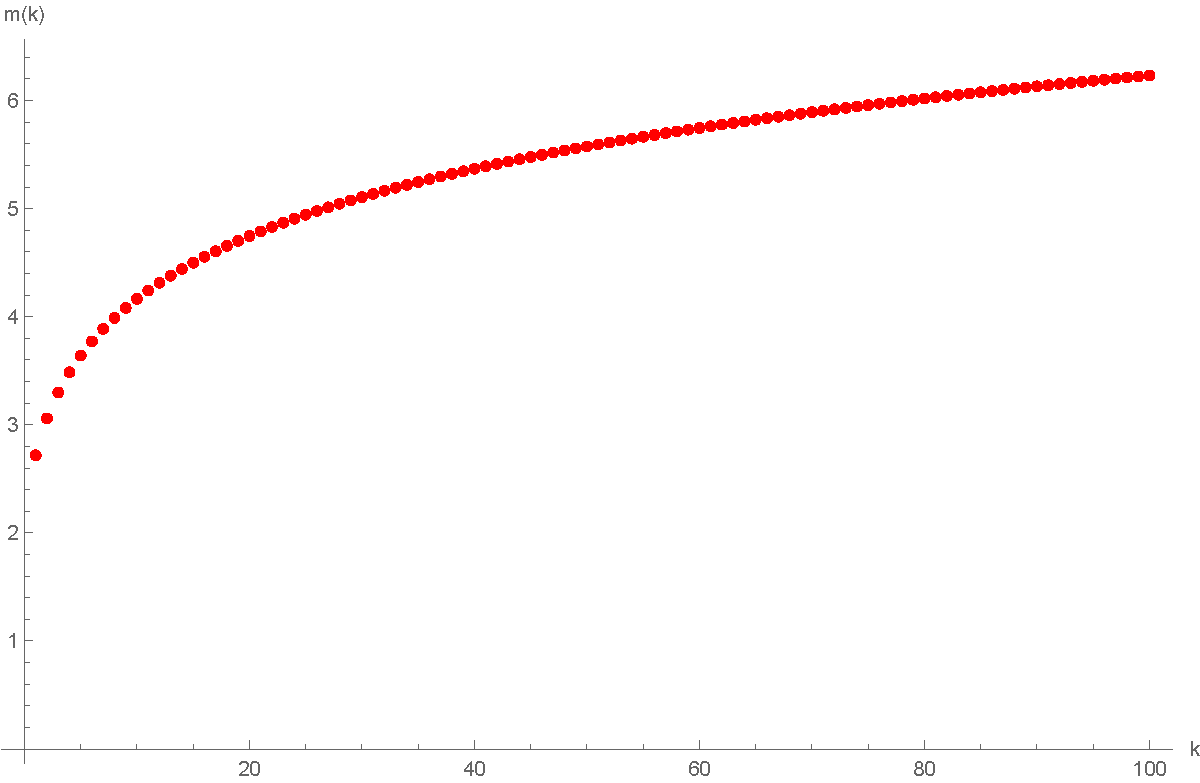
\includegraphics[scale=0.3]{Images/first100rmfc.pdf}} % Optional title page image, comment this line to remove it
\institute{Department of Mathematics,\\ University of Mumbai}

\date{\today}
%------------------------------------------------

\begin{document}

%------------------------------------------------

\begin{frame}
	\maketitle % Automatically created using the information in the commands above
\end{frame}

%----------------------------------------------------------------------------------------
%	 SECTION 1
%----------------------------------------------------------------------------------------



\begin{frame}
	\frametitle{Table of Contents}
	\tableofcontents
\end{frame}

\section{Background/Motivation}
\begin{frame}{Abelian categories}
	\[ \textbf{Abelian} \subseteq \textbf{Karoubian} \subseteq \textbf{Pre-Abelian} \subseteq \textbf{Additive} \subseteq \textbf{Ab-Enriched}\]
\note{The category of projective modules over any ring is the Karoubi envelope of its full subcategory of free modules.

	An additive category is an Ab-Enriched category which has all finite biproducts.

A kernel is a pullback of a morphism $f:A \to B$ and the unique morphism from $0 \to B$. Provided initials and pullbacks exist.

A pre-abelian category is an additive category with all morphism having kernels and cokernels.

An abelian category is a pre-abelian categories for which each mono is a kernel and each epic is a cokernel.}
\end{frame}
%\begin{frame}[fragile,allowframebreaks]{Riemann–Roch}
%	\begin{theorem}[Classical Riemann–Roch]
%		Let $X$ be a connected compact Riemann surface of genus $g$, and let $D$ be a divisor on $X$. Then
%		\[
%		\ell(D)-\ell(K_X-D)=\deg D + 1 - g,
%		\]
%		where $\ell(D)=\dim_{\Bbb C}H^{0}(X,\mathcal O_X(D))$ and $K_X$ is a canonical divisor.
%	\end{theorem}
%	
%	\begin{definition}[Divisor]
%		A \emph{divisor} on $X$ is a finite formal sum $D=\sum_{p\in X} n_p\,p$ with $n_p\in\Bbb Z$.
%		Its \emph{degree} is $\deg D=\sum n_p$.
%	\end{definition}
%	
%	\begin{definition}[Line bundle of a divisor]
%		For a divisor $D$, $\mathcal O_X(D)$ is the holomorphic line bundle of meromorphic
%		functions whose divisor of zeros and poles is bounded by $D$.
%	\end{definition}
%	
%	\begin{definition}[Genus]
%		The \emph{genus} of $X$ is $g=\dim_{\Bbb C}H^{1}(X,\mathcal O_X)$.
%	\end{definition}
%	
%	\begin{definition}[$\ell(D)$]
%		$\ell(D)$ denotes $\dim_{\Bbb C} H^{0}(X,\mathcal O_X(D))$.
%	\end{definition}
%\end{frame}

%\begin{frame}[allowframebreaks, fragile]{Grothendieck–Riemann–Roch}
%	\begin{theorem}[Grothendieck–Riemann–Roch]
%		Let $f\colon X\to Y$ be a proper morphism between smooth quasi-projective varieties over a field of characteristic $0$,
%		and let $E$ be a vector bundle on $X$.  In the rational Chow ring $A^{*}(Y)\otimes\Bbb Q$,
%		\[
%		\mathrm{ch}\!\bigl(f_{!}E\bigr)\cdot\mathrm{td}(T_Y)=
%		f_{*}\!\bigl(\mathrm{ch}(E)\cdot\mathrm{td}(T_X)\bigr),
%		\]
%		where $f_{!}E=\sum_{i}(-1)^{i}R^{i}f_{*}E$ in $K_0(Y)$.
%	\end{theorem}
%	
%	\begin{definition}[$K_0(X)$]
%		$K_{0}(X)$ is the Grothendieck group of vector bundles on $X$: the abelian group generated by isomorphism
%		classes of vector bundles modulo relations $[E]-[E']+[E'']=0$ for every short exact sequence
%		$0\to E'\to E\to E''\to0$.
%	\end{definition}
%	
%	\begin{definition}[Chern character]
%		The \emph{Chern character} $\mathrm{ch}\colon K_{0}(X)\to A^{*}(X)\otimes\Bbb Q$
%		is the unique ring homomorphism that sends a line bundle $L$ to $\exp(c_1(L))$.
%	\end{definition}
%	
%	\begin{definition}[Todd class]
%		$\mathrm{td}(T_X)\in A^{*}(X)\otimes\Bbb Q$ is the multiplicative characteristic class
%		determined by the Chern classes of the tangent bundle $T_X$.
%	\end{definition}
%	
%	\begin{block}{Why $K_0$?}
%		Grothendieck needed a functorial target for the push-forward $f_{!}$ that is additive in
%		exact sequences; $K_0$ achieves this, whereas classical Chow and Picard groups do not.
%	\end{block}
%\end{frame}


\section{Geometry \( \to \) Algebra }

\begin{frame}{Swan's theorem}
	\begin{theorem}
		Let $X$ be a compact Hausdorff space. Then the section functor $\Gamma$ induces an equivalence of categories $\mathcal{VB}(X) \simeq \mathrm{Proj}(C(X))$.
	\end{theorem}
	\note{	\begin{definition}[Equivalence of categories]\index{Equivalence of categories}
			Two categories $\mathcal{C},\mathcal{D}$ are said to be equivalent if there exist functors $E:\mathcal{C}\rightleftarrows \mathcal{D}:F$ and a pair of natural \textit{isomorphisms} $\alpha: 1_\mathbf{C} \to F \circ E$ and $\beta: 1_\mathbf{D} \to E \circ F$. 
			This is a weaker condition than isomorphism of categories in which we have an actual equality instead of natural isomorphism.
		\end{definition}
	}
\end{frame}

\begin{frame}[allowframebreaks]{Swan's theorem: Sketch of the proof}
	\begin{itemize}
		\item \textbf{Key Lemma:} For any vector bundle $E$ over a compact space $X$, there exists another vector bundle $E'$ such that their Whitney sum is a trivial bundle:
		\[ E \oplus E' \simeq X \times \mathbf{k}^n \]
		\item The section functor $\Gamma$ is additive, so it turns Whitney sums into direct sums of modules:
		\[ \Gamma(E) \oplus \Gamma(E') \simeq \Gamma(X \times \mathbf{k}^n) \simeq C(X)^n \]
		\item Since $\Gamma(E)$ is a direct summand of a free module ($C(X)^n$), it is, by definition, a finitely generated projective $C(X)$-module. This confirms the functor $\Gamma$ maps into the correct target category.
	\end{itemize}
	\pagebreak
	\begin{itemize}
		\item $\mathcal{VB}_T(X)$: The full subcategory of \textbf{trivial} vector bundles.
		\item $\mathrm{Free}(C(X))$: The full subcategory of finitely generated \textbf{free} $C(X)$-modules.
	\end{itemize}
	The section functor provides a straightforward equivalence between these two simple categories:
	\[ \Gamma_T: \mathcal{VB}_T(X) \stackrel{\simeq}{\longrightarrow} \mathrm{Free}(C(X)) \]
	
	\pagebreak
	
	\textbf{The Main Idea: The Karoubian Envelope.}
	A category is \textbf{Karoubian} if all its idempotent morphisms split. Both $\mathcal{VB}(X)$ and $\mathrm{Proj}(C(X))$ are Karoubian. The Karoubian envelope is a universal way to "complete" an additive category by formally adding objects that split idempotents.
	
	\begin{itemize}
		\item From Part 1, every vector bundle is a direct summand of a trivial one. This means $\mathcal{VB}(X)$ is precisely the \textbf{Karoubian envelope of $\mathcal{VB}_T(X)$}.
		
		\item By definition, every projective module is a direct summand of a free one. This means $\mathrm{Proj}(C(X))$ is precisely the \textbf{Karoubian envelope of $\mathrm{Free}(C(X))$}.
	\end{itemize}
	
	\textbf{The Punchline:} A fundamental property of the Karoubian envelope is that an equivalence of categories lifts to an equivalence of their envelopes.
\end{frame}

\begin{frame}{Motivation for higher algebraic K groups}
	Topological K theory obey Eilenberg-Steenrod minus dimensionality, i.e. generalized cohomology theory.
	\begin{itemize}
		\item Homotopic
		\item Exactness
		\item Excision
		\item Additivity
	\end{itemize}
	
\end{frame}

\section{Simplicial Homotopy theory}

\begin{frame}[fragile]{Model categories}
		\begin{definition}[Model category]
		$\mathcal{C}$ with 3 distinguished classes of morphisms $(\mathcal{W, F ,C})$:
		\begin{itemize}
			\item $\mathcal{C}$ is bicomplete.
			\item $\mathcal{W}$ has the `2-out-of-3'.
			\item $(\mathcal{C},\mathcal{F}\cap \mathcal{W})$ and $(\mathcal{C}\cap \mathcal{W},\mathcal{F})$ both form weak factorization systems.
		\end{itemize}
	\end{definition}	
\end{frame}
\note{	\begin{definition}[Serre fibration]
		A map $\rho: X \to Y$ is called a Serre fibration if for every finite CW complex $A$, the map $\rho$ has the right lifting property with respect to the inclusion map $A \times 0  \to A \times [0,1].$
	\end{definition}
	
	\begin{proposition}[Classical Quillen model structure on $\mathbf{Top}$]
		Consider morphisms $f:X\to Y $ in $\mathbf{Top}$. We can define a model structure on $\mathbf{Top}$ with the following distinguished classes of maps $(\mathcal{W,F,C})$ as such,
		\begin{enumerate}
			\item $f \in \mathcal{W}$ if $f$ is a weak homotopy equivalence in $\mathbf{Top}$, i.e., $f:X \to Y$ is a map whose induced homomorphisms on homotopy groups (for every basepoint) are bijective.
			\item $f \in \mathcal{F}$ if $f$ is a Serre fibration.
			\item $f \in \mathcal{C}$ if $f$ is a retract of a relative cell complex. A relative cell complex is just an arbitrary cell complex not necessarily countable like in the case of CW complexes.
		\end{enumerate}
\end{proposition}}
\begin{frame}[fragile, allowframebreaks]{Homotopy}
	
	\begin{definition}[Path space object]
		Let $\mathcal{C}$ be a model category with the distinguished class of maps $(\mathcal{W,F,C})$. Then define the path object for $X \in \mathcal{C}$ as the object obtained in its factorization of the diagonal morphism $$\Delta: X \xrightarrow{(1_X,1_X)} X \times X.$$
		\[\begin{tikzcd}
			& {\mathrm{Path}(X)} \\
			X && {X\times X}
			\arrow["{(r_0,r_1) \in \mathcal{F}}", from=1-2, to=2-3]
			\arrow["{\lambda \in \mathcal{W}}", from=2-1, to=1-2]
			\arrow["{\Delta}", from=2-1, to=2-3]
		\end{tikzcd}\]
	\end{definition}
	\pagebreak
	\begin{definition}[Cylinder object]\index{Cylinder object}
		Let $\mathcal{C}$ be a model category with the distinguished class of maps $(\mathcal{W,F,C})$. Then define the cylinder object for $X \in \mathcal{C}$ as the object obtained from the factorization of the codiagonal ``folding'' morphism $\nabla: X \sqcup X \xrightarrow{[1_X,1_X]} X$.
		\[\begin{tikzcd}
			& {\mathrm{Cyl}(X)} \\
			{X\sqcup X} && X
			\arrow["{\rho\in \mathcal{W}}", from=1-2, to=2-3]
			\arrow["{(l_0,l_1)\in\mathcal{C}}", from=2-1, to=1-2]
			\arrow["\nabla"', from=2-1, to=2-3]
		\end{tikzcd}\]
	\end{definition}
	\pagebreak
	\begin{definition}[Fibrant objects]\index{(Co)Fibrant objects}
		Let $\mathcal{C}$ be a model category with distinguished classes of maps $(\mathcal{W,F,C})$. An object $A \in \mathcal{C}$ is said to be fibrant if the unique mapping into the terminal object $(f: A \to 1) \in \mathcal{F}$.
	\end{definition}

	\begin{definition}[Cofibrant objects]
		As defined above, an object $B \in \mathcal{C}$ is said to be cofibrant if the unique mapping from the initial object $(g:0 \to B) \in \mathcal{C}$.
	\end{definition}
	
	
		\begin{example}
		\begin{enumerate}
			\item The canonical example is that Kan complexes in the classical model structure of simplicial sets are fibrant. All simplicial sets are cofibrant in the standard model structure on the category of simplicial sets.
			\item All topological spaces in the classical model structure of topological spaces are fibrant.
			\item In the projective model category of chain complexes the complexes with projective objects are cofibrant and the complexes with injective objects are fibrant.
		\end{enumerate}
		
	\end{example}
	
%	\begin{proposition}\label{prop-fib-acycfib}
%		If $X \in \mathcal{C}$ a model category is fibrant then the map $\rho=(\rho_0, \rho_1): \mathrm{Path}(X) \to X \times X$ is a fibration and also the induced maps  $\rho_0, \rho_1$ are individually acyclic fibrations into $X$.
%		
%		Dually we have the map from $X \sqcup X \to \mathrm{Cyl}(X)$ is a cofibration and the individual maps from $X \to \mathrm{Cyl}(X)$ are acyclic cofibrations provided $X$ is a cofibrant object.
%	\end{proposition}
%	
		\begin{definition}[Left homotopy in a model category]\index{Homotopy}
		Let $\mathcal{C}$ be a model category and objects $X,Y \in \mathcal{C}$.
		
		If we have \( f, g: X \to Y \) then a left homotopy if it exists is a diagram of the following sort 
		
		\( H_l: f \rightarrow g \) is a morphism \( H_l: \mathrm{Cyl}(X) \to Y \) making the below diagram commute.
		\[\begin{tikzcd}
			X \\
			{\mathrm{Cyl}(X)} && Y \\
			X
			\arrow["{l_1}", from=1-1, to=2-1]
			\arrow["f", from=1-1, to=2-3]
			\arrow["{H_l}", from=2-1, to=2-3]
			\arrow["{l_0}"', from=3-1, to=2-1]
			\arrow["g"', from=3-1, to=2-3]
		\end{tikzcd}\]
		
	\end{definition}
	\begin{definition}[Right homotopy in a model category]
		Let $\mathcal{C}$ be a model category and objects $X,Y \in \mathcal{C}$.
		
		If we have \( f, g: X \to Y \) then a right homotopy if it exists is a diagram of the following sort 
		
		\( H_r: f \rightarrow g \) is a morphism, \( H_r: X \to \mathrm{Path}(Y) \) making the below diagram commute.
		
		\[\begin{tikzcd}
			&& Y \\
			X && {\mathrm{Path}(Y)} \\
			&& Y
			\arrow["{r_1}"', from=2-3, to=1-3]
			\arrow["f", from=2-1, to=1-3]
			\arrow["{H_r}", from=2-1, to=2-3]
			\arrow["g"', from=2-1, to=3-3]
			\arrow["{r_0}", from=2-3, to=3-3]
		\end{tikzcd}\]
	\end{definition}
	
	\begin{lemma}
		Let $\mathcal{C}$ be a model category and $f,g : X \to Y$ be morphisms. If $X$ is cofibrant then a left homotopy implies existence of a right homotopy independent on choice of path space object.
	\end{lemma}
	
	\begin{corollary}
		If as defined above $X$ is cofibrant and $Y$ is fibrant then left and right homotopies between them coincide and form an equivalence relation.
	\end{corollary}
\end{frame}

\begin{frame}[allowframebreaks, fragile]{Simplicial sets}
		\begin{definition}[Simplex/finite ordinal category]\index{Category!Simplex/finite ordinal ($\Delta$)}
		We refer to $\Delta$ as the simplex category. It is defined by the objects of finite non empty, totally ordered sets,
		\[ [n]=\{0 \to 1 \to \cdots \to n\} \]
		maps between these objects are order preserving, i.e. non decreasing maps between totally ordered sets.
		$f: [m] \to [n]$ is a map such that $f(0) \leq f(1) \leq \cdots \leq f(m)$.
		
		The category formed by all such finite non empty, totally ordered sets and all the mappings between them is referred to as the simplex category $\Delta$.
	\end{definition}
	\pagebreak
		\begin{example}
		\( f:[1]\to[5] \), defined by \( f(0 \to 1)= 2 \to 4 \)
		$f:[2] \to [5]$, defined by $f(0 \to 1 \to 2) = 2 \to 3 \to 4$.
		\( f:[3] \to [5] \), defined by \( f(0 \to 1 \to 2 \to 3)=3 \to 4 \to 4 \to 5 \).
		
	\end{example}	
	\begin{example}
		
		$g:[4] \to [2]$ defined by $g(0 \to 1 \to 2\to 3 \to 4) = 0\to 0 \to 1 \to 1 \to 1.$		
	\end{example}
		\pagebreak
	Note that all morphisms in $\Delta$ are generated by a natural family of functions called coface and degeneracy maps defined as below.
	\begin{definition}[Coface maps]
		$d^i:[n-1] \to [n]$ the injection which misses the $i^\mathrm{th}$ element in $[n]$.
		
		Explicitly, for $0 \leq i \leq n$
		\[
		d^i(k) =
		\begin{cases}
			k, & k < i \\
			k + 1, & k \geq i
		\end{cases}
		\]
	\end{definition}
	\begin{definition}[Codegeneracy maps]
		$s^i:[n+1]\to[n]$ the surjection which maps two elements to $i$.
		\[
		s^i(k) =
		\begin{cases}
			k, & k \leq i \\
			k - 1, & k > i
		\end{cases}
		\]
	\end{definition}
	
	These obey the relations,
	\begin{align*}
		d^j d^i &= d^i d^{j-1}, & i < j \\
		s^j s^i &= s^i s^{j+1}, & i \leq j \\
		s^j d^i &= 1, & i = j, j+1 \\
		s^j d^i &= d^i s^{j-1}, & i < j \\
		s^j d^i &= d^{i-1} s^j, & i > j+1.
	\end{align*}
\pagebreak
	\begin{definition}[Simplicial set]
		A simplicial set is a functor $X: \Delta^\mathrm{op} \to \mathbf{Set}$, i.e. presheaves on $\Delta$. It comprises of a collection of sets $X_n =X([n])$ which we to call the set of $n-$simplices of $X$ with maps between them corresponding naturally with maps in $\Delta$.
	\end{definition}
	
	
	
	Furthermore corresponding to coface maps from $[n-1] \to [n]$ in $\Delta$ we get a family of face maps between simplices $d_i:X_n \to X_{n-1}$, $0\leq i \leq n$.
	
	The degeneracy maps corresponding to codegeneracy maps $ [n+1] \to n$ as a family of maps $s_i: X_n \to X_{n+1}$.
	
	Defined as such,
	\begin{align*}
		d_i &= X d^i : X_n \to X_{n-1} & 0 \leq i \leq n \\
		s_i &= X s^i : X_n \to X_{n+1} & 0 \leq i \leq n
	\end{align*}
	
	
	These obey the standard relations,
	\begin{align*}
		d_id_j &= d_{j-1}d_i, &i <j\\
		s_is_j&=s_{j+1}s_i &i \leq j\\
		d_is_j&=1, &i=j,j+1\\
		d_is_j&=s_{j-1}d_i,& i<j\\
		d_is_j&=s_jd_{i-1},& i>j+1
	\end{align*}
	
	The face maps $d_i$ can be understood as mapping each $n$-simplex $x\in X_n$ to $n+1$ many $n-1$ simplicies $d_i(x)$ $0\leq i \leq n$ in $X_{n-1} $, the $i^\mathrm{th}$ face does not contain the $i^{\mathrm{th}}$ vertex of $x$. 
	
	Similarly for degeneracy maps $s_i$ we can understand it as mapping $x \in X_n $ to $n+1$ many $n+1$ simplicies in $X_{n+1} $ and $s_i(x)$ has $x$ as its $i^{\mathrm{th}} $ and $i+1^{\mathrm{th}}$ face. 
	
	\pagebreak


\begin{proposition}
	Any simplicial set can be expressed as a colimit of standard n simplicies, where the indexing category is the category of simplices. In particular for $X \in \mathbf{sSet}$ we have, \[ \colim_{x \in X_n}\Delta[n] \cong X. \]
\end{proposition}

	\begin{definition}[Simplicial objects in arbitrary categories]
	For $\mathcal{C}$ an arbitrary category a simplical object in $\mathcal{C}$ is a functor $C: \Delta^{op} \to \mathcal{C}$.
\end{definition}
\note{\begin{theorem}[Density theorem]
		Let $\mathcal{C}$ be a small category, every object $X \in \mathbf{Sets}^{\mathcal{C}^{\mathrm{op}}}$ is a colimit of representable functors for a index category $J$ the category of elements of $X$,
		\[ \colim_{j \in J} y C_j \cong X .\]
\end{theorem}

\begin{lemma}[Yoneda]\index{Yoneda lemma}
	For a locally small category\index{Category!Locally small} $\mathcal{C}$ \footnote{Locally small implies each homset is indeed a small set (i.e. not a proper class). This is a weaker condition than just the category being small which means the collection of objects is a small set \index{Category! Small}.}, an object $A \in \mathcal{C}$ and a functor $F$  in the functor category $\mathbf{Sets}^{\mathcal{C}^\mathrm{op}}$ there exists an isomorphism,\[ \Hom_{\mathbf{Sets}^{\mathcal{C}^\mathrm{op}}}(yA, F) \cong FA.\]
	
	Where $y: \mathcal{C} \to \mathbf{Sets}^{\mathcal{C}^\mathrm{op}}$ is the Yoneda embedding defined as, $$y(A):\Hom_\mathcal{C}(-, A).$$ For $A$ an object of $\mathcal{C}$ and, $$y(f:A \to B):\Hom_\mathcal{C}(-,f): \Hom_\mathcal{C}(-,A) \to \Hom_\mathcal{C}(-,B).$$
	\end{lemma}}
\pagebreak
\begin{definition}[Geometric realization of a standard $n$-simplical set]
	We define a functor $|.|:\mathbf{sSet} \to \mathbf{Top}$ as such. Send each standard $n$ simplex $\Delta[n]$ to the standard $n$-toplogical simplex. In particular,
	\[ |\Delta[n]|=\{ (x_0,\dots,x_{n+1}) | 0 \leq x_i \leq 1, \sum x_i=1 \} \subset \R^{n+1}. \]
\end{definition}
	We can then define the geometric realization of a standard \(n\)-simplex as \(|\Delta[n]|=\Delta_n\) where \(\Delta_n\) the standard topological \(n\)-simplex.
\pagebreak
	\begin{figure}[!htb]
	\centering
	\[\begin{tikzcd}
		& 2 && 2 \\
		&& 2 \\
		0 &&&& 1 \\
		& 0 && 1 \\
		& 0 && 1
		\arrow[""{name=0, anchor=center, inner sep=0}, from=3-1, to=1-2]
		\arrow[""{name=1, anchor=center, inner sep=0}, from=3-5, to=1-4]
		\arrow[""{name=2, anchor=center, inner sep=0}, from=4-2, to=2-3]
		\arrow[""{name=3, anchor=center, inner sep=0}, from=4-2, to=4-4]
		\arrow[""{name=4, anchor=center, inner sep=0}, from=4-4, to=2-3]
		\arrow[""{name=5, anchor=center, inner sep=0}, from=5-2, to=5-4]
		\arrow["{d_1}"', shorten <=7pt, shorten >=7pt, Rightarrow, from=2, to=0]
		\arrow["{d_2}", shorten <=4pt, shorten >=4pt, Rightarrow, from=3, to=5]
		\arrow["{d_0}", shorten <=7pt, shorten >=7pt, Rightarrow, from=4, to=1]
	\end{tikzcd}\]
	\caption{Face maps for 2-simplex}
	\label{fig:facemaps}
\end{figure}

\begin{figure}[!htb]
	\centering
	\[\begin{tikzcd}
		& 2 \\
		&& {} && {} \\
		0 && 1 && 0 && 1
		\arrow[squiggly, from=2-3, to=2-5]
		\arrow[""{name=0, anchor=center, inner sep=0}, from=3-1, to=1-2]
		\arrow[""{name=1, anchor=center, inner sep=0}, from=3-1, to=3-3]
		\arrow[from=3-3, to=1-2]
		\arrow[from=3-5, to=3-7]
		\arrow["{s_1}"', curve={height=-6pt}, shorten <=6pt, shorten >=6pt, Rightarrow, from=0, to=1]
	\end{tikzcd}\]
	\caption{Degeneracy maps for 2-simplex}
	\label{fig:degenmaps}
\end{figure}

\end{frame}


\begin{frame}[allowframebreaks,fragile]{Classifying spaces}
	\begin{definition}[Nerve of a small category]
		Let $\mathcal{C}$ be a small category we define its nerve as the following simplicial set $N(\mathcal{C})_0=\mathrm{Ob}(\mathcal{C})$, $\mathcal{C}$ and $N(\mathcal{C})_1 = \mathrm{Mor}(\mathcal{C})$ and $N(\mathcal{C})_k=\{(f_1,\ldots,f_k)| f_i \in \mathrm{Mor}(\mathcal{C})\}$ consists of $k-$tuples of composable arrows, face maps defined as $$d_i(f_1,\ldots, f_i,f_{i+1}, \ldots, f_k)=(f_1,\ldots f_i\circ f_{i+1}, \ldots, f_k)$$ and degeneracy maps defined as $$s_j=(f_1,\ldots,f_k)=(f_1,\ldots,f_{j-1}, 1, f_j,\ldots,f_k).$$
	\end{definition}
	
	In a concise manner the nerve is simply the simplicial set consisting of $n$-simplicies of the form $N(\mathcal{C}_n):=\Hom([n], \mathcal{C})$.
	
	\begin{figure}[!htb]
		\centering
		
		
		% Gradient Info
		
		\tikzset {_iz92akyfm/.code = {\pgfsetadditionalshadetransform{ \pgftransformshift{\pgfpoint{89.1 bp } { -108.9 bp }  }  \pgftransformscale{1.32 }  }}}
		\pgfdeclareradialshading{_8bfavxm42}{\pgfpoint{-72bp}{88bp}}{rgb(0bp)=(1,1,1);
			rgb(0bp)=(1,1,1);
			rgb(25bp)=(0.61,0.61,0.61);
			rgb(400bp)=(0.61,0.61,0.61)}
		\tikzset{every picture/.style={line width=0.75pt}} %set default line width to 0.75pt        
		
		\begin{tikzpicture}[x=0.75pt,y=0.75pt,yscale=-1,xscale=1]
			%uncomment if require: \path (0,310); %set diagram left start at 0, and has height of 310
			
			%Shape: Circle [id:dp009025913185087164] 
			\path  [shading=_8bfavxm42,_iz92akyfm] (379.19,125.88) .. controls (379.19,86.99) and (410.72,55.47) .. (449.6,55.47) .. controls (488.49,55.47) and (520.02,86.99) .. (520.02,125.88) .. controls (520.02,164.77) and (488.49,196.3) .. (449.6,196.3) .. controls (410.72,196.3) and (379.19,164.77) .. (379.19,125.88) -- cycle ; % for fading 
			\draw   (379.19,125.88) .. controls (379.19,86.99) and (410.72,55.47) .. (449.6,55.47) .. controls (488.49,55.47) and (520.02,86.99) .. (520.02,125.88) .. controls (520.02,164.77) and (488.49,196.3) .. (449.6,196.3) .. controls (410.72,196.3) and (379.19,164.77) .. (379.19,125.88) -- cycle ; % for border 
			
			%Curve Lines [id:da9761986007165273] 
			\draw  [dash pattern={on 0.84pt off 2.51pt}]  (379.19,125.88) .. controls (380.08,104.9) and (520.08,104.9) .. (520.02,125.88) ;
			%Curve Lines [id:da37207250146051574] 
			\draw    (379.19,125.88) .. controls (378.93,145.18) and (519.79,144.9) .. (520.02,125.88) ;
			%Curve Lines [id:da5571298015729296] 
			\draw    (449.6,55.47) .. controls (429.5,55.75) and (429.22,195.47) .. (449.6,196.3) ;
			%Curve Lines [id:da8854464399728328] 
			\draw  [dash pattern={on 0.84pt off 2.51pt}]  (449.6,55.47) .. controls (468.93,55.75) and (468.36,195.47) .. (449.6,196.3) ;
			%Straight Lines [id:da9972704527950889] 
			\draw    (129.19,126.21) -- (198.19,195.21) ;
			\draw [shift={(199.6,196.63)}, rotate = 225] [color={rgb, 255:red, 0; green, 0; blue, 0 }  ][line width=0.75]    (10.93,-3.29) .. controls (6.95,-1.4) and (3.31,-0.3) .. (0,0) .. controls (3.31,0.3) and (6.95,1.4) .. (10.93,3.29)   ;
			%Straight Lines [id:da7565729134262409] 
			\draw    (270.02,126.21) -- (201.02,195.21) ;
			\draw [shift={(199.6,196.63)}, rotate = 315] [color={rgb, 255:red, 0; green, 0; blue, 0 }  ][line width=0.75]    (10.93,-3.29) .. controls (6.95,-1.4) and (3.31,-0.3) .. (0,0) .. controls (3.31,0.3) and (6.95,1.4) .. (10.93,3.29)   ;
			%Straight Lines [id:da5238988037401515] 
			\draw    (270.02,126.21) -- (186.77,139.85) ;
			\draw [shift={(184.8,140.17)}, rotate = 350.7] [color={rgb, 255:red, 0; green, 0; blue, 0 }  ][line width=0.75]    (10.93,-3.29) .. controls (6.95,-1.4) and (3.31,-0.3) .. (0,0) .. controls (3.31,0.3) and (6.95,1.4) .. (10.93,3.29)   ;
			%Straight Lines [id:da7020252864051173] 
			\draw    (129.19,126.21) -- (198.19,57.21) ;
			\draw [shift={(199.6,55.8)}, rotate = 135] [color={rgb, 255:red, 0; green, 0; blue, 0 }  ][line width=0.75]    (10.93,-3.29) .. controls (6.95,-1.4) and (3.31,-0.3) .. (0,0) .. controls (3.31,0.3) and (6.95,1.4) .. (10.93,3.29)   ;
			%Straight Lines [id:da10254818035410218] 
			\draw    (184.8,140.17) -- (199.26,57.77) ;
			\draw [shift={(199.6,55.8)}, rotate = 99.95] [color={rgb, 255:red, 0; green, 0; blue, 0 }  ][line width=0.75]    (10.93,-3.29) .. controls (6.95,-1.4) and (3.31,-0.3) .. (0,0) .. controls (3.31,0.3) and (6.95,1.4) .. (10.93,3.29)   ;
			%Straight Lines [id:da11176389907972806] 
			\draw    (199.6,196.63) -- (185.31,142.11) ;
			\draw [shift={(184.8,140.17)}, rotate = 75.31] [color={rgb, 255:red, 0; green, 0; blue, 0 }  ][line width=0.75]    (10.93,-3.29) .. controls (6.95,-1.4) and (3.31,-0.3) .. (0,0) .. controls (3.31,0.3) and (6.95,1.4) .. (10.93,3.29)   ;
			%Straight Lines [id:da5957088382370499] 
			\draw    (270.02,126.21) -- (201.02,57.21) ;
			\draw [shift={(199.6,55.8)}, rotate = 45] [color={rgb, 255:red, 0; green, 0; blue, 0 }  ][line width=0.75]    (10.93,-3.29) .. controls (6.95,-1.4) and (3.31,-0.3) .. (0,0) .. controls (3.31,0.3) and (6.95,1.4) .. (10.93,3.29)   ;
			%Straight Lines [id:da48122644038923923] 
			\draw    (129.19,126.21) -- (182.86,139.68) ;
			\draw [shift={(184.8,140.17)}, rotate = 194.09] [color={rgb, 255:red, 0; green, 0; blue, 0 }  ][line width=0.75]    (10.93,-3.29) .. controls (6.95,-1.4) and (3.31,-0.3) .. (0,0) .. controls (3.31,0.3) and (6.95,1.4) .. (10.93,3.29)   ;
			%Straight Lines [id:da8775980959118528] 
			\draw  [dash pattern={on 0.84pt off 2.51pt}]  (129.19,126.21) -- (213.69,109.98) ;
			\draw [shift={(215.66,109.6)}, rotate = 169.12] [color={rgb, 255:red, 0; green, 0; blue, 0 }  ][line width=0.75]    (10.93,-3.29) .. controls (6.95,-1.4) and (3.31,-0.3) .. (0,0) .. controls (3.31,0.3) and (6.95,1.4) .. (10.93,3.29)   ;
			%Straight Lines [id:da14708687520763286] 
			\draw  [dash pattern={on 0.84pt off 2.51pt}]  (270.02,126.21) -- (217.57,110.18) ;
			\draw [shift={(215.66,109.6)}, rotate = 16.99] [color={rgb, 255:red, 0; green, 0; blue, 0 }  ][line width=0.75]    (10.93,-3.29) .. controls (6.95,-1.4) and (3.31,-0.3) .. (0,0) .. controls (3.31,0.3) and (6.95,1.4) .. (10.93,3.29)   ;
			%Straight Lines [id:da017637905326172376] 
			\draw  [dash pattern={on 0.84pt off 2.51pt}]  (215.66,109.6) -- (200.25,59.51) ;
			\draw [shift={(199.66,57.6)}, rotate = 72.9] [color={rgb, 255:red, 0; green, 0; blue, 0 }  ][line width=0.75]    (10.93,-3.29) .. controls (6.95,-1.4) and (3.31,-0.3) .. (0,0) .. controls (3.31,0.3) and (6.95,1.4) .. (10.93,3.29)   ;
			%Straight Lines [id:da32673657468438044] 
			\draw  [dash pattern={on 0.84pt off 2.51pt}]  (215.66,109.6) -- (199.97,194.66) ;
			\draw [shift={(199.6,196.63)}, rotate = 280.45] [color={rgb, 255:red, 0; green, 0; blue, 0 }  ][line width=0.75]    (10.93,-3.29) .. controls (6.95,-1.4) and (3.31,-0.3) .. (0,0) .. controls (3.31,0.3) and (6.95,1.4) .. (10.93,3.29)   ;
			
			% Text Node
			\draw (377.19,125.88) node [anchor=east] [inner sep=0.75pt]    {$a$};
			% Text Node
			\draw (464.18,107.67) node [anchor=south west] [inner sep=0.75pt]    {$b$};
			% Text Node
			\draw (522.02,125.88) node [anchor=west] [inner sep=0.75pt]    {$c$};
			% Text Node
			\draw (433.27,136.88) node [anchor=south east] [inner sep=0.75pt]    {$d$};
			% Text Node
			\draw (449.6,199.7) node [anchor=north] [inner sep=0.75pt]    {$e$};
			% Text Node
			\draw (449.2,49.27) node [anchor=south] [inner sep=0.75pt]    {$f$};
			% Text Node
			\draw (127.19,126.21) node [anchor=east] [inner sep=0.75pt]    {$a$};
			% Text Node
			\draw (214.18,108) node [anchor=south west] [inner sep=0.75pt]    {$b$};
			% Text Node
			\draw (272.02,126.21) node [anchor=west] [inner sep=0.75pt]    {$c$};
			% Text Node
			\draw (186.07,132.41) node [anchor=south east] [inner sep=0.75pt]    {$d$};
			% Text Node
			\draw (199.6,200.03) node [anchor=north] [inner sep=0.75pt]    {$e$};
			% Text Node
			\draw (199.2,49.6) node [anchor=south] [inner sep=0.75pt]    {$f$};
			% Text Node
			\draw (190.29,235.74) node [anchor=north west][inner sep=0.75pt]    {$\mathcal{C} \ \ \ \ \ \ \ \ \ \ \ \ \ \ \ \ \ \ \ \ \ \ \ \ \ \ \ \ \ \ \ \ \ \ \ \ \ \ \ \ \ \ \  \ \ |B\mathcal{C} |$};
			
			
		\end{tikzpicture}
		
		
		
		\caption{Example of a geometric realization of a simplex. Note here $C$ is not a groupoid so the corresponding classifying space is not a Kan complex.}
		\label{fig:exofnerve}
	\end{figure}
	
	
	

\end{frame}

\begin{frame}[allowframebreaks, fragile]{Kan complexes}
	\begin{definition}[Horn of a standard $n$-simplex]
		Given a standard $n$-simplex $\Delta[n]$ the $k^\text{th}$ horn is denoted as $\Lambda_k[n]$ for $0 \leq k \leq n$. It is a subset of $\Delta[n]$ generated by all faces except the $k^\text{th}$ face.
	\end{definition}
	
	
	
	
	\begin{definition}[Kan complexes]
		$X \in \mathbf{sSets}$ is a Kan complex if all horns on $X$ can be filled. In particular this means that any map $\Lambda_k[n] \to X$ can be extended to a map $\Delta[n] \to X$.
	\end{definition}
	
	\begin{definition}[Kan fibration]\index{Kan fibration}
		A simplicial map \( f: X\to Y \) is said to be a Kan fibration if it has the right lifting property against all horn inclusions, i.e. the lift \( h \) below always exists.
		\[\begin{tikzcd}
			{\Lambda_k[n]} & X \\
			{\Delta[n]} & Y
			\arrow[from=1-1, to=1-2]
			\arrow[from=1-1, to=2-1]
			\arrow["f", from=1-2, to=2-2]
			\arrow[dashed, from=2-1, to=1-2]
			\arrow[from=2-1, to=2-2]
		\end{tikzcd}\]
	\end{definition}
		\begin{proposition}
		A small category $\mathcal{C}$ is a groupoid if and only if $B\mathcal{C}$ is a Kan complex.
	\end{proposition}
	
	\begin{figure}[!htb]
		\centering
		\[\begin{tikzcd}
			& 3 &&&& 3 \\
			0 && 1 & \subset & 0 && 1 \\
			& 2 &&&& 2 \\
			& {\Lambda^2[3]} &&&& {\Delta[3]}
			\arrow[from=2-1, to=3-2]
			\arrow[from=2-3, to=3-2]
			\arrow[from=2-5, to=1-6]
			\arrow[from=2-5, to=2-7]
			\arrow[from=2-5, to=3-6]
			\arrow[from=2-7, to=1-6]
			\arrow[from=2-7, to=3-6]
			\arrow[from=3-2, to=1-2]
			\arrow[from=3-6, to=1-6]
		\end{tikzcd}\]
		\caption{Example of a horn of a $3$-simplex}
		\label{fig:horn}
	\end{figure}
\end{frame}

\begin{frame}[allowframebreaks,fragile]{\( \mathrm{Ex}^\infty \) functor}
		\begin{definition}[Barycentric subdivision of a standard simplicial set]\index{Barycentric subdivision}
		For \( \Delta[n] \) define its barycentric subdivison \( \mathrm{sd}\Delta[n] \) as the nerve of the poset of non-degenerate simplicies \( \mathrm{nd}\Delta[n] \), i.e. \( \mathrm{sd} \Delta[n]=B \mathrm{nd}\Delta[n]. \) 
	\end{definition}
	For an arbitrary simplicial set \( X \) we proceed via the colimit of its representatives as one may expect, \[ \mathrm{sd}X = \mathrm{colim}_{x \in X_n} \mathrm{sd}(\Delta[n]) .\] This notion of a barycentric subdivision is exactly the same as that commonly encountered in standard algebraic topology.
	
	\begin{figure}[!htb]
		\centering
		\[\begin{tikzcd}
			&& 2 \\
			& 02 & 012 & 12 \\
			0 && 01 && 1
			\arrow[from=1-3, to=2-2]
			\arrow[from=1-3, to=2-3]
			\arrow[from=1-3, to=2-4]
			\arrow[from=2-2, to=2-3]
			\arrow[from=2-4, to=2-3]
			\arrow[from=3-1, to=2-2]
			\arrow[from=3-1, to=2-3]
			\arrow[from=3-1, to=3-3]
			\arrow[from=3-3, to=2-3]
			\arrow[from=3-5, to=2-3]
			\arrow[from=3-5, to=2-4]
			\arrow[from=3-5, to=3-3]
		\end{tikzcd}\]
		\caption{Example of the barycentric subdivision of \(\Delta[2]\).}
		\label{fig:bary}
	\end{figure}
	\begin{definition}[Ex functor]
		For \( X \in \mathbf{sSets} \) define \( \mathrm{Ex} \) levelwise as \( \mathrm{Ex}(X)_n = \Hom(\mathrm{sd}\Delta[n],X) \).
	\end{definition}
	
	Since we know \( X_n \cong \Hom(\Delta[n],X) \) we have by construction \( \mathrm{Ex} \) is right adjoint to \( \mathrm{sd} \).
	
	There is a natural map \( X \to \mathrm{Ex}(X) \). Iterating this procedure repeatedly and taking a colimit of the diagram,\[ X \to \mathrm{Ex}(X) \to \mathrm{Ex}^2(X) \to \dots. \]
	We obtain the simplicial set \( \mathrm{Ex}^\infty X \).\index{$\mathrm{Ex}^\infty$ functor}
	
	The elements of \( \mathrm{Ex}^\infty(X)_1 \) consist of `zig-zags' of morphisms in \( X \).
	\[\begin{tikzcd}
		& \bullet && \bullet && {} \\
		\bullet && \bullet && \bullet && {}
		\arrow[from=1-2, to=2-1]
		\arrow[from=1-2, to=2-3]
		\arrow[dotted, no head, from=1-4, to=1-6]
		\arrow[from=1-4, to=2-3]
		\arrow[from=1-4, to=2-5]
		\arrow[dotted, no head, from=2-5, to=2-7]
	\end{tikzcd}\]
	

	\begin{theorem}
		For any simplicial set \( X \), \( \mathrm{Ex}^\infty(X) \) is a Kan complex.
	\end{theorem}
\end{frame}

\begin{frame}[allowframebreaks,fragile]{Simplicial homotopy groups}
		Simplicial homotopy groups are defined only for fibrant objects.
			
		With this in mind we define the simplicial homotopy groups of Kan complexes as such.
		
		We begin with a notion of a `simplicial sphere'.
		\begin{definition}[Boundary of a standard simplical set]\index{Boundary of a simplicial set}
			Let \( \Delta[n]\in \mathbf{sSets} \) denote the standard \( n \) simplicial set. We denote its boundary as \( \partial \Delta[n] \) and it is defined as the subsimplicial set of \( \Delta[n] \) consisting of all non-degenerate \( m \) simplicies for \( m <n \). That is to say all except its unique non-degenerate  \( n \) simplex.
		\end{definition}
		
		The way to visualize this is to think of the fact that the geometric realization of \( \partial \Delta[n] \) is precisely homotopic to \( S^{n-1} \).
		
		\begin{definition}[Simplicial homotopy groups]\index{Simplicial homotopy groups}
			Let \( X \in \mathbf{sSets} \) be a Kan complex, choose some vertex \( v \in X_0 \).
			
			Define \( \pi_0(X)  \) as the set of simplicial homotopy classes of vertices of \( X \).
			
			Define the underlying set of \(\pi_n(X,v) \) as the set of homotopy classes of morphisms \( \alpha: \Delta[n] \to X \) such that these take the boundary of \( \Delta[n] \) to the point \( x \), i.e. there exists a commutative diagram as such.
			\[\begin{tikzcd}
				{\Delta[n]} & X \\
				{\partial \Delta[n]} & {\Delta[0]}
				\arrow["\alpha", from=1-1, to=1-2]
				\arrow[from=2-1, to=1-1]
				\arrow[from=2-1, to=2-2]
				\arrow["v",from=2-2, to=1-2]
			\end{tikzcd}\]
			
		\end{definition}
		
		The group operation is given as follows. Let \( f, g \) be distinct representatives in \( \pi_n(X,v) \).
		
		Consider the following \( n \)-simplices in \( X \),
		\[ \begin{cases}
			v_i &= v, 0 \leq i \leq n-2,\\
			v_{n-1} &= \alpha,\\
			v_{n+1} &= \beta.
		\end{cases} \]
		Note that \( d_i v_j=d_{j-1}v_i \) for \( i<j, i,j \neq n. \) Therefore these \( v_i \) define a simplical map, \[ (v_0,\dots,v_{n-1},-,v_{n+1}): \Lambda_n[n+1] \to X \] which since \( X \) is fibrant gives us a lift \( \theta \).
		\[\begin{tikzcd}
			{\Delta_n[n+1]} &&& X \\
			{\Delta[n+1]}
			\arrow["{ (v_0,\dots,v_{n-1},-,v_{n+1})}", from=1-1, to=1-4]
			\arrow[from=1-1, to=2-1]
			\arrow["\theta"', dashed, from=2-1, to=1-4]
		\end{tikzcd}\]
		Note that,
		\begin{align*}
			\partial(d_n\theta) &= (d_0d_n\theta, \dots, d_{n-1}d_n\theta, d_nd_n\theta) \\
			&= (d_{n-1}d_0\theta, \dots, d_{n-1}d_{n-1}\theta, d_nd_{n+1}\theta) \\
			&= (v, \dots, v),
		\end{align*}
		Therefore, \( d_n\theta \) is an element of \( \pi_n(X,v) \).
		We define the group product as \( [f]\cdot [g]=[d_n\theta] \).
		
		It still remains to show that the choice of \( d_n\theta \) is independent of the representatives and the lift \( \theta \). Also that the product indeed defines a group. For this see Goerss-Jardine [7.1, 7.2].
\end{frame}

\begin{frame}[allowframebreaks,fragile]{A Quillen equivalence}
	\begin{proposition}
		A simplicial map \( f:X\to Y \) is a weak equivalence (classically) if and only if \( \mathrm{Ex}^\infty (f): \mathrm{Ex}^\infty (X) \to \mathrm{Ex}^\infty (Y)\) is a simplicial homotopy equivalence.
	\end{proposition}
	
	\begin{proposition}[Classical model structure on simplicial sets]
		Denoted as \( \mathbf{sSets}_\mathrm{Quillen} \) the classical model structure on simplicial sets consists of the following classes of morphisms
		\begin{enumerate}
			\item Weak equivalences are given as simplicial weak equivalences.
			\item Fibrations are given as Kan fibrations.
			\item Cofibrations are given by monomorphisms (levelwise injections).
		\end{enumerate}
	\end{proposition}
	
	In this model structure the fibrant objects are precisely Kan complexes and every simplicial set is cofibrant. 
	
	There exists a Quillen adjunction between the classical model structure on simplicial sets and the classical model structure on topological spaces. The Quillen adjunction is induced by none other than the singularisation-geometric realisation adjunction.
\end{frame}

\section{Quillen \( Q \) construction}
\begin{frame}[allowframebreaks,fragile]{Exact categories}
	\begin{definition}[Exact category]\label{defexactcat}
		An exact category (sometimes referred to as a Quillen exact category) is a pair $\mathcal{(E},E)$ for $\mathcal{E}$ an additive category which is a full subcategory of some abelian category $\mathcal{A}$. Along with a family of sequences $E$ of the form, \[ 0 \to A \to B \to C \to 0. \] Which are short exact sequences in $\mathcal{A}$ and if in a sequence of the above form $A, C \in \mathcal{E}$ then $B $ is isomorphic to some element which is in $\mathrm{Ob}(C)$, (i.e. it is closed under extensions).
	\end{definition}
	\pagebreak
	\begin{example}
		\begin{itemize}
			\item 	For \(A\) a commutative ring with unity, the collection of finitely generated projective \( A \) modules forms an exact category. 
			\item Every abelian category is trivially exact over itself.
			\item Torsion free abelian groups over the category of abelian groups is exact but not abelian.
		\end{itemize}
	\end{example}
	\pagebreak
	
	\begin{definition}[$K_0$ for an exact category $\mathcal{E}$]\label{def:k0exact}
		$K_0(\mathcal E)$ is generated by the isomorphism classes $[B]$ for each $B \in \mathrm{Ob}(\mathcal{E})$ and a relation of $[B]=[A]+[C]$ for all short exact sequences, \[ 0 \to A \to B \to C \to 0.\]
	\end{definition}
	\note{{Why \([B] = [A] + [C]\) is Natural}
		Short exact sequences describe how objects are built. The relation \([B] = [A] + [C]\) reflects that \(B\) is an extension of \(C\) by \(A\). In the split case, \(B \cong A \oplus C\), so additivity becomes obvious. Doubly so when split}
\end{frame}
\begin{frame}[allowframebreaks,fragile]{\( Q \) construction of an exact category}
	Suppose that \(\mathcal{E}\) is an exact category. Define an equivalence relation on all diagrams
	
	\[
	A \twoheadleftarrow P \rightarrowtail B
	\]
	
	by saying that the top and bottom pictures in the diagram
	
	\[\begin{tikzcd}
		& {P'} \\
		A && B \\
		& P
		\arrow[two heads, from=1-2, to=2-1]
		\arrow[tail, from=1-2, to=2-3]
		\arrow["\cong", dashed, from=1-2, to=3-2]
		\arrow[two heads, from=3-2, to=2-1]
		\arrow[tail, from=3-2, to=2-3]
	\end{tikzcd}\]
	
	are equivalent if the displayed isomorphism exists, making the diagram commute.
	
	The category \( Q\mathcal{E} \)\index{Q-construction} has for objects all objects of \( \mathcal{E} \). The morphisms \( A \to B \) are the equivalence classes of the pictures above. Composition is defined by pullback:
	
	\[\begin{tikzcd}
		&& {Q\times_MP} \\
		& Q && P \\
		A && B && C
		\arrow["p"', two heads, from=1-3, to=2-2]
		\arrow["i", tail, from=1-3, to=2-4]
		\arrow["\lrcorner"{anchor=center, pos=0.125, rotate=-45}, draw=none, from=1-3, to=3-3]
		\arrow[two heads, from=2-2, to=3-1]
		\arrow[tail, from=2-2, to=3-3]
		\arrow[two heads, from=2-4, to=3-3]
		\arrow[tail, from=2-4, to=3-5]
	\end{tikzcd}\]
	
	
	In order for composition in \( Q\mathcal{E}\) to be coherent we expect the morphism \( i \) and \( p \) as shown above to actually be admissible monics and epis respectively.
	\begin{proposition}Admissible monics are closed under pullbacks along admissible epis, and admissible epis are closed under pushouts along admissible monics.
	\end{proposition}
\end{frame}
\begin{frame}[allowframebreaks,fragile]{Equivalence of groupoids}
	\begin{theorem}
		There is an equivalence of groupoids $GQ\mathcal{E} \cong K_0(\mathcal{E})$.
	\end{theorem}	
	\pagebreak
	
	\begin{alertblock}{Proof Strategy}
		We construct functors in both directions and show they are mutually inverse.
		\begin{enumerate}
			\item A functor $\psi: GQ\mathcal{E} \to K_0(\mathcal{E})$.
			\item A functor $\psi^{-1}: K_0(\mathcal{E}) \to GQ\mathcal{E}$.
		\end{enumerate}
	\end{alertblock}
	
	
	
	\textbf{Functor 1: Constructing $\psi: GQ\mathcal{E} \to K_0(\mathcal{E})$}
	
	We first define a map $\psi_*$ from the generating morphisms of $Q\mathcal{E}$ to the group $K_0(\mathcal{E})$.
	
	\begin{itemize}
		\item \textbf{On Admissible Epimorphisms ($\twoheadrightarrow$):} For an epi $p: P \twoheadrightarrow B$, we define its image as the class of its kernel in $K_0$.
		\[ \psi_*(p) = [\ker p] \in K_0(\mathcal{E}) \]
		This choice correctly preserves composition, as the proof shows that for a composite epi $b \circ p$, we get $\psi_*(b \circ p) = \psi_*(b) + \psi_*(p)$.
		
		
		
		\item \textbf{On Admissible Monomorphisms ($\rightarrowtail$):} For a monic $i: A \rightarrowtail P$, we define its image to be trivial.
		\[ \psi_*(i) = [0] \in K_0(\mathcal{E}) \]
		
		\item By the universal property of the free groupoid ($G$), since $K_0(\mathcal{E})$ is itself a groupoid, our map $\psi_*$ on generators extends uniquely to the required functor $\psi: GQ\mathcal{E} \to K_0(\mathcal{E})$.
	\end{itemize}
	
	
	
	\textbf{Functor 2: Constructing $\psi^{-1}: K_0(\mathcal{E}) \to GQ\mathcal{E}$}
	
	\begin{itemize}
		\item The group $K_0(\mathcal{E})$ is a groupoid with one object. We map this single object to the zero object $0 \in GQ\mathcal{E}$.
		
		\item A morphism in $K_0(\mathcal{E})$ is an element $[B]$. We map it to the canonical morphism in $GQ\mathcal{E}$ given by the sequence $0 \rightarrowtail B \twoheadrightarrow B$.
		
		\item This functor respects the group law. The proof shows that the defining relation of $K_0$ from a short exact sequence $0 \to A \to C \to B \to 0$ is preserved. That is, the construction using a pullback diagram confirms:
		\[ \psi^{-1}([C]) = \psi^{-1}([A]) \circ \psi^{-1}([B]) \]
		
	\end{itemize}
	
	
	
	\textbf{Conclusion}
	
	The two functors $\psi$ and $\psi^{-1}$ are constructed to be mutually inverse up to natural isomorphism. For instance, applying them in sequence shows that $\psi(\psi^{-1}([P])) = [P]$. Thus, they establish the desired equivalence of groupoids.
	\hfill 
	
	
\end{frame}
\begin{frame}[allowframebreaks,fragile]{Higher K groups with the \( Q \) construction}
		\begin{corollary}
		There is an isomorphism of groups \( K_0(\mathcal{E}) \cong \pi_1(BQ\mathcal{E},0) \)
	\end{corollary}
	\begin{proof}
		We have an equivalence of groupoids,
		\(  GP_*(BQ \mathcal{E}) \simeq K_0(\mathcal{E}). \)
		Since the groupoid $K_0(\mathcal{E})$ has only one object, it is connected. The equivalence implies that the groupoid $GP_*(BQ\mathcal{E})$ is also connected.
		
		The fundamental group $\pi_1(BQ\mathcal{E}, 0)$ is, by definition, the automorphism group of the object $0$ in the fundamental groupoid. Therefore,
		\[ \pi_1(BQ\mathcal {E}, 0) \cong \operatorname{Aut}_{K_0(\mathcal{E})}(*) \cong K_0(\mathcal{E}). \]
	\end{proof}
	
	This finally motivates the following definition of \( K \)-groups via the \( Q \)-construction.
	\begin{definition}[Higher $K$-groups]
		\(K_n(\mathcal{E})= \pi_{n+1}(BQ\mathcal{E},0)\)
	\end{definition}
\end{frame}

\section{Waldhausen \( s_\bullet \) construction}
\begin{frame}[allowframebreaks,fragile]{Waldhausen \( s_\bullet \) construction}
	\begin{definition}[Waldhausen \( s_\bullet \)-construction]\index{Waldhausen \( s_\bullet \) construction}
		Let $\mathcal{E}$ be an exact category with its distinguished class of exact sequences $E$. For each integer $n \geq 0$, let $\mathrm{Arr}(\mathbf{n})$ be the arrow category of the ordinal $n$.
	\end{definition}
		Define $s_n(\mathcal{E})$ to be the set of all functors
		\[ P: \mathrm{Arr}(n) \to \mathcal{E} \]
		such that the following conditions hold:
		\begin{enumerate}
			\item $P(i, i) \cong 0$ for all $0 \leq i \leq n$.
			\item For any sequence $i \leq j \leq k$ in $n$, the sequence induced by the morphisms $(i,j) \to (i,k)$ and $(i,k) \to (j,k)$ in $\mathrm{Arr}(\mathbf{n})$, namely
			\[ 0 \to P(i, j) \rightarrowtail P(i, k) \twoheadrightarrow P(j, k) \to 0 \]
			is an exact sequence in $E$.
		\end{enumerate}
		A functor $P$ satisfying these conditions is called an exact functor in this context.
		
		These sets form a simplicial set $s_\bullet(\mathcal{E})$ whose $n$-simplices are the elements of $s_n(\mathcal{E})$.

	
	This simplicial set $s_\bullet(\mathcal{E})$ is the Waldhausen \( s_\bullet \)-construction for the exact category $\mathcal{E}$.
	
	\begin{example}
		The following is a picture of exact \( P:\mathrm{Arr}(\mathbf{3}) \to \mathcal{E} \). Note that all the squares are pullback+pushout diagrams (bicartesian) since two parallel admissible epis share kernels.
		\[\begin{tikzcd}[column sep=small]
			&&& {P(0,3)} \\
			&& {P(0,2)} && {P(1,3)} \\
			& {P(0,1)} && {P(1,2)} && {P(2,3)} \\
			0 && 0 && 0 && 0
			\arrow[two heads, from=1-4, to=2-5]
			\arrow[tail, from=2-3, to=1-4]
			\arrow[two heads, from=2-3, to=3-4]
			\arrow[two heads, from=2-5, to=3-6]
			\arrow[tail, from=3-2, to=2-3]
			\arrow[two heads, from=3-2, to=4-3]
			\arrow[tail, from=3-4, to=2-5]
			\arrow[two heads, from=3-4, to=4-5]
			\arrow[two heads, from=3-6, to=4-7]
			\arrow[tail, from=4-1, to=3-2]
			\arrow[tail, from=4-3, to=3-4]
			\arrow[tail, from=4-5, to=3-6]
		\end{tikzcd}\]
	\end{example}
	To recover the more familar definition of the Waldhausen construction note that the above diagram is generated by the string of monics \[0\rightarrowtail P(0,1)\rightarrowtail P(0,2) \rightarrowtail P(0,3) \] by attaching all cokernels.
	
\end{frame}
\begin{frame}[allowframebreaks,fragile]{Segal edgewise subdivision}
	\begin{definition}[Join of elements in a poset]
		For two elements in a poset their join is just their coproduct.
	\end{definition}
	\begin{example}
		When \( \mathbf{n} \) is a ordinal number consider \( \mathbf{n}^\mathrm{op} \) then \( \mathbf{n}^\mathrm{op} \vee \mathbf{n} \cong \mathbf{2n+1} \). This can be seen in the following diagram.
		\[\begin{tikzcd}
			0 & 1 & 2 & \cdots & n \\
			0 & 1 & 2 & \dots & n
			\arrow[from=1-1, to=1-2]
			\arrow[from=1-2, to=1-3]
			\arrow[from=1-3, to=1-4]
			\arrow[from=1-4, to=1-5]
			\arrow[from=2-1, to=1-1]
			\arrow[from=2-2, to=2-1]
			\arrow[from=2-3, to=2-2]
			\arrow[from=2-4, to=2-3]
			\arrow[from=2-5, to=2-4]
		\end{tikzcd}\]
	\end{example}
	This defines a functor \( e:\Delta \to \Delta \), as \( e(\mathbf{n}) = \mathbf{n}^\mathrm{op} \vee \mathbf{n} .\)
	
	\begin{definition}[Segal's edgewise subdivision of a simplicial set]\index{Segal edgewise subdivision}
		For \( X \in \mathbf{sSets} \) consider the functor \( X^e=Xe^{\mathrm{op}} \), i.e. \[ X_n^e=X(\mathbf{n}^\mathrm{op} \vee \mathbf{n}) \].
		The face and degeneracy maps are defined as such,
		\begin{align*}
			d^e_i&=d_{n-i} d_{n+1+i}:X_{\mathbf{2n+1}} \to X_{\mathbf{2n-1}}\\
			s^e_j&=s_{n-j} s_{n+1+j}:X_{\mathbf{2n+1}} \to X_{\mathbf{2n+3}}	
		\end{align*}
		
	\end{definition}
	
	\begin{example}
		Consider \( \Delta[2] \) the standard \( 2\)-simplex.
		
		\( \Delta[2]_0^e=\Delta[2]_1=\{(0\to0), (0\to1), (0 \to 2), (1 \to 1), (1 \to 2), (2 \to 2)\} \)
		\( \Delta[2]_1^e=\Delta[2]_3=\{ (0 \to 0 \to 0 \to 0), (0 \to 0 \to 0 \to 1), (0 \to 0 \to 0 \to 2), (0 \to 0 \to 1 \to 1), (0 \to 0 \to 1 \to 2), (0 \to 0 \to 2 \to 2), (0 \to 1 \to 1 \to 1), (0 \to 1 \to 1 \to 2), (0 \to 1 \to 2 \to 2), (0 \to 2 \to 2 \to 2), (1 \to 1 \to 1 \to 1), (1 \to 1 \to 1 \to 2), (1 \to 1 \to 2 \to 2), (1 \to 2 \to 2 \to 2), (2 \to 2 \to 2 \to 2) \} \)
		
		With an appropriate abuse of notation we see a much clearer picture of the subdivision \( \Delta[2]^e \)as such. Each chain \( (f_1,f_2,f_3,f_4) \) corresponds to \( (f_2,f_3) \to (f_1,f_4) \)
		\[\begin{tikzcd}
			&& {(1,1)} \\
			& {(0,1)} && {(1,2)} \\
			{(0,0)} && {(0,2)} && {(2,2)}
			\arrow[from=1-3, to=2-2]
			\arrow[from=1-3, to=2-4]
			\arrow[from=1-3, to=3-3]
			\arrow[from=2-2, to=3-3]
			\arrow[from=2-4, to=3-3]
			\arrow[from=3-1, to=2-2]
			\arrow[from=3-1, to=3-3]
			\arrow[from=3-5, to=2-4]
			\arrow[from=3-5, to=3-3]
		\end{tikzcd}\]
	\end{example}
	\begin{theorem}[A simplicial set is weakly equivalent to its Segal subdivision] \label{th:segalsubdivweakeq}
		The natural map \( \omega:X^e \to X \) is a weak equivalence.
	\end{theorem}
\end{frame}
\begin{frame}[allowframebreaks,fragile]{Relationship between Quillens and Waldhausens constructions}
	\begin{definition}
		For an exact category \( \mathcal{E} \) define $\mathrm{Iso}_n(\mathcal{E})$ as the category whose objects are all strings
		\[ Q \colon Q_0 \xrightarrow{\cong} Q_1 \xrightarrow{\cong} \dots \xrightarrow{\cong} Q_n \]
		of isomorphisms of length $n$. The morphisms are natural transformations.
	\end{definition}
	
	This can be understood as a natural groupoid-ification of an exact category.
	
	\begin{lemma}\label{lem:isoequivexact}
		Let $\mathcal{E}$ be an exact category. Define functors $f: \mathcal{E} \to \mathrm{Iso}_n(\mathcal{E})$ by $P \mapsto (P \xrightarrow{1_P} P \xrightarrow{1_P} \dots \xrightarrow{1_P} P)$ and $g: \mathrm{Iso}_n(\mathcal{E}) \to \mathcal{E}$ by $(Q_0 \xrightarrow{q_0} Q_1 \to \dots \xrightarrow{q_{n-1}} Q_n) \mapsto Q_0$. Then $f$ and $g$ form an exact equivalence of categories.
	\end{lemma}
	
		\begin{definition}[Simplicial exact category]
		Define \( S_\bullet(\mathcal{E}) \) as a category whose objects are exact functors \( P:\mathrm{Arr} (\mathbf{n}) \to \mathcal{E}\) as previously defined. The morphisms in the category are natural transformations between functors.
	\end{definition}
	
	
	We consider the groupoidification of the exact categories $S_\bullet(\mathcal{E})^e$ and $BQ\mathcal{E}$.
	
	The simplicial set map $\pi \colon s_\bullet(\mathcal{E})^e \to BQ\mathcal{E}$ is the object-level part of a map of simplicial groupoids, also denoted $\pi$:
	\[ \pi \colon \mathrm{Iso}(S_\bullet(\mathcal{E}))^e \to \mathrm{Iso}(BQ\mathcal{E}) \]
	As a map of simplicial groupoids, this $\pi$ acts on objects as previously defined and also provides a consistent mapping for the natural isomorphisms (the morphisms within these groupoids).
	
	\begin{lemma}\label{lem:isoSisoBQEeq}
		The morphism of groupoids \( \pi_n: \mathrm{Iso}(S_\bullet (\mathcal{E}))^e_n \to \mathrm{Iso}(BQ\mathcal{E})_n \) induces a weak equivalence between their nerves \( B\mathrm{Iso}(S_\bullet (\mathcal{E}))^e_n \simeq B\mathrm{Iso}(BQ\mathcal{E})_n \)
	\end{lemma}
	
		\begin{theorem}[Equivalence between Waldhausen's \( s_\bullet \) and Quillen Q construction]
		For an exact category \( \mathcal{E} \), there exist weak equivalences \( s_\bullet(\mathcal{E}) \simeq s_\bullet(\mathcal{E})^e \simeq BQ \mathcal{E}\).
	\end{theorem}
	
	\pagebreak
	\begin{alertblock}{Proof Strategy}
		The proof establishes the two weak equivalences in the chain separately.
		\begin{enumerate}
			\item The first equivalence, $s_\bullet(\mathcal{E}) \simeq s_\bullet(\mathcal{E})^e$, is a general fact about Segal's edgewise subdivision.
			\item The second equivalence, $s_\bullet(\mathcal{E})^e \simeq BQ\mathcal{E}$, is the core of the proof and uses the "2-out-of-3" property for weak equivalences.
		\end{enumerate}
	\end{alertblock}
	
	\pagebreak
	
	\textbf{Part 1: Equivalence via Edgewise Subdivision}
	
	\begin{itemize}
		\item The map $\omega: s_\bullet(\mathcal{E})^e \to s_\bullet(\mathcal{E})$ is the natural projection from the edgewise subdivision to the original simplicial set.
		\item \textbf{Key Fact (Thm 6.1.5):} For any simplicial set $X$, the map from its edgewise subdivision $X^e \to X$ is a weak equivalence.
		\item Therefore, the first link in our chain, $s_\bullet(\mathcal{E}) \simeq s_\bullet(\mathcal{E})^e$, holds.
	\end{itemize}
	
	
	
	\textbf{Part 2: Equivalence via the "2-out-of-3" Property}
	
	We need to show that the map $\pi: s_\bullet(\mathcal{E})^e \to BQ\mathcal{E}$ constructed in the text is a weak equivalence. We use the following commutative diagram:
	
	\[
	\begin{tikzcd}
		s_\bullet(\mathcal{E})^e \arrow{r}{\eta}[swap]{\simeq} \arrow{d}{\pi} & B(\text{Iso}(S_\bullet(\mathcal{E})^e)) \arrow{d}{B(\tilde{\pi})}[swap]{\simeq} \\
		B Q \mathcal{E} \arrow{r}{\eta'}[swap]{\simeq} & B(\text{Iso}(B Q \mathcal{E}))
	\end{tikzcd}
	\]
	
	The strategy is to show the other three maps are weak equivalences.
	
	\begin{enumerate}
		\item[\textbf{(a)}] The right vertical map $B(\tilde{\pi})$ is a weak equivalence.
		\begin{itemize}
			\item This follows from Lemma 6.2.4, which shows that $\tilde{\pi}$ is an \textit{equivalence of categories} at each level. An equivalence of categories induces a weak equivalence on their nerves (classifying spaces).
		\end{itemize}
		
		
		
		\item[\textbf{(b)}] The top horizontal map $\eta$ is a weak equivalence.
		\begin{itemize}
			\item This map includes the objects of the exact category $S_n(\mathcal{E})^e$ into the nerve of its groupoid of isomorphisms. By Lemma 6.2.2, an exact category is equivalent to its category of isomorphism strings, so their nerves are weakly equivalent.
		\end{itemize}
		
		\item[\textbf{(c)}] The bottom horizontal map $\eta'$ is a weak equivalence for the exact same reason, since $BQE_k$ is an exact category for each level $k$.
	\end{enumerate}
	
	
	
	\textbf{Conclusion}
	
	Since the maps $\eta$, $\eta'$, and $B(\tilde{\pi})$ are all weak equivalences, the 2-out-of-3 property for weak equivalences implies that our map $\pi: s_\bullet(\mathcal{E})^e \to BQ\mathcal{E}$ must also be a weak equivalence.
	
	Combining both parts, we have the full chain of equivalences: $ s_\bullet(\mathcal{E}) \simeq s_\bullet(\mathcal{E})^e \simeq BQ\mathcal{E} $.
	\hfill \( \square \)
\end{frame}
\begin{frame}[allowframebreaks,fragile]{Additivity theorem}
	
	
	
	\begin{theorem}[Additivity Theorem]
		\label{thm:Additivity_manual_proper_no_id_cmd_generic_label_v2}
		Let $\mathcal{E}$ be an exact category. The simplicial set map
		\[ (t_*, s_*) : s_{\bullet}\mathrm{Ex}(\mathcal{E}) \to s_{\bullet}\mathcal{E} \times s_{\bullet}\mathcal{E} \]
		is a weak equivalence. Here $t_*$, $s_*$ are induced by taking the kernel and cokernel, respectively.
	\end{theorem}
	
	\begin{alertblock}{Proof Strategy}
		The proof works by interpreting this map as a map between two fibrations over the common base space $s.\mathcal{E}$ and then showing it induces a weak equivalence on the fibers.
	\end{alertblock}
	
	\textbf{Step 1: The Fibrations}
	
	We consider two fibrations over $s.\mathcal{E}$. The first is the map $s_*: s.\mathrm{Ex}(\mathcal{E}) \to s.\mathcal{E}$ which projects a diagram of exact sequences to its diagram of cokernels. The second is the standard projection from the product, $pr_2: s.\mathcal{E} \times s.\mathcal{E} \to s.\mathcal{E}$. The map $(t_*, s_*)$ respects these projections and is therefore a map of fibrations.
	
	\textbf{Step 2: The Fibers}
	
	To show the map of total spaces is a weak equivalence, we analyze the map it induces on the homotopy fibers over an arbitrary point $P \in s.\mathcal{E}$. The fiber of $s_*$ over $P$ is the space of exact sequences whose cokernels are given by $P$, which we denote $s_*^{-1}(P)$. The fiber of $pr_2$ over $P$ is simply $s.\mathcal{E} \times \{P\}$, weakly equivalent to $s.\mathcal{E}$. The map on the fibers is thus given by $t_*: s_*^{-1}(P) \to s.\mathcal{E}$, which takes an exact sequence with cokernel $P$ to its kernel.
	
	\textbf{Step 3: The Crucial Lemma}
	
	The argument hinges on the key technical result from the text (Lemma 6.3.1), which states that the fiber map
	\[ t_*: s_*^{-1}(P) \longrightarrow s.\mathcal{E} \]
	is a weak equivalence for any $P \in s.\mathcal{E}$. This essentially means that specifying the cokernel of an exact sequence places no homotopical constraint on its kernel.
	
	\textbf{Step 4: Conclusion}
	
	The map of fibrations $(t_*, s_*)$ must be a weak equivalence on the total spaces precisely because it is a weak equivalence on both the base space (it's the identity) and on all the fibers (by the lemma). This completes the sketch.
	

\end{frame}
\begin{frame}[allowframebreaks,fragile]{\( K \)-theory spectrum	}
		\begin{definition}[Stable Equivalence of K-theory Spectra]
		A map $\phi_*: K(\mathcal{E}_1) \to K(\mathcal{E}_2)$ of symmetric spectra, induced by an exact functor $f: \mathcal{E}_1 \to \mathcal{E}_2$, is a {stable equivalence} if it induces isomorphisms on all stable homotopy groups:
		\[ \pi_n(\phi_*): \pi_n(K(\mathcal{E}_1)) \xrightarrow{\cong} \pi_n(K(\mathcal{E}_2)) \quad \text{for all } n \in \mathbb{Z}. \]
		The stable homotopy groups $\pi_n(K(\mathcal{E}))$ are defined as $\mathrm{colim}_k \pi_{n+k}(K(\mathcal{E})^k)$. A map of symmetric spectra is a stable equivalence if it is an isomorphism in the stable homotopy category. For K-theory spectra, $\pi_n K(\mathcal{E})$ often corresponds to the classical $K_n$-groups of $\mathcal{E}$ for $n \ge 0$ and are zero for $n < 0$.
	\end{definition}
\end{frame}
\begin{frame}[allowframebreaks,fragile]{Resolution/D\'evissage}
		\begin{theorem}[Resolution Theorem]
		Suppose that $\mathcal{P}$ is full and closed under extensions in the exact category $\mathcal{E}$, and that $\mathcal{P}$ and $\mathcal{E}$ satisfy the following conditions,
			\end{theorem}
		\begin{enumerate}
			\item All admissible epis \( P \twoheadrightarrow P' \) between objects of \( \mathcal{P} \) in \( \mathcal{E} \) are admissible epis of \( \mathcal{P} \).
			\item Given any admissible epi \( f:Q \twoheadrightarrow P \) with \( P \in \mathcal{P} \), there is a commutative diagram as such,
			\[\begin{tikzcd}
				{P'} \\
				Q & P
				\arrow[from=1-1, to=2-1]
				\arrow[two heads, from=1-1, to=2-2]
				\arrow["f"', two heads, from=2-1, to=2-2]
			\end{tikzcd}\]
		\end{enumerate} Then the inclusions
		\[ \mathcal{P} \subset \mathcal{P}_1 \subset \mathcal{P}_2 \subset \dots \subset \mathcal{P}_\infty \]
		induce stable equivalences
		\[ K(\mathcal{P}) \simeq K(\mathcal{P}_1) \simeq K(\mathcal{P}_2) \simeq \dots \simeq K(\mathcal{P}_\infty). \]

	\pagebreak
	\begin{theorem}[D\'evissage Theorem]
		Suppose that $\mathcal{B}$ is a non-empty subcategory of a small abelian category $\mathcal{A}$ which is closed under taking finite direct sums, subobjects and quotients in $\mathcal{A}$. Suppose that every object $Q$ of $\mathcal{A}$ has a finite filtration
		\[ 0 = F_{-1} \rightarrowtail F_0 \rightarrowtail F_1 \rightarrowtail \dots \rightarrowtail F_n = Q \]
		with all filtration quotients $F_i/F_{i-1} \in \mathcal{B}$. Then the inclusion $i : \mathcal{B} \to \mathcal{A}$ induces a stable equivalence $K(\mathcal{B}) \simeq K(\mathcal{A})$.
	\end{theorem}
\end{frame}

\nocite{karoubi2008k}
\nocite{quillenhigherktheoryI}
\nocite{quillen1967homotopical}
\nocite{Goerss_Jardine_2009}	
%------------------------------------------------
\section{References}
\begin{frame}[allowframebreaks]
        \frametitle{References}
        
        \bibliographystyle{unsrt}
    \tiny{\bibliography{references.bib}}
\end{frame}
%------------------------------------------------
\begin{frame}
    \textbf{\Huge{Thank you}}
\end{frame}
%------------------------------------------------


\end{document}
